%!TEX root = ../Pflichtenheft.tex

\chapter{Benutzeroberfläche}
\label{chap:ui}

\section{Haupseite und Buchung}

Die Startseite der Anwendung ist in \ref{fig:startseite} dargestellt.
Auf dieser haben NutzerInnen die Möglichkeit, dem Raum zu buchen oder auf andere Ansichten zu wechseln.

Der Banner in allen Ansichten zeigt den aktuellen Raumstatus an.
Insbesondere wird dadurch die Priorität der aktuellen Buchung mithilfe der Farbe des Banners angezeigt.

Rechts in dieser Ansicht befindet sich ein Kalender, der die aktuelle Woche und die Buchungen in diesem Zeitraum anzeigt.
Die Buchungen sind farblich nach Priorität gekennzeichnet, weitere Informationen können durch Klicken auf die Buchung eingesehen werden.

Neben dieser Möglichkeit, den Raum zu buchen, gibt es einen Anmeldebutton und einen separaten Buchungsbutton für NutzerInnen,
für die die Verwendung des Kalenders Probleme bereitet.
\begin{figure}[ht]
    \centering
    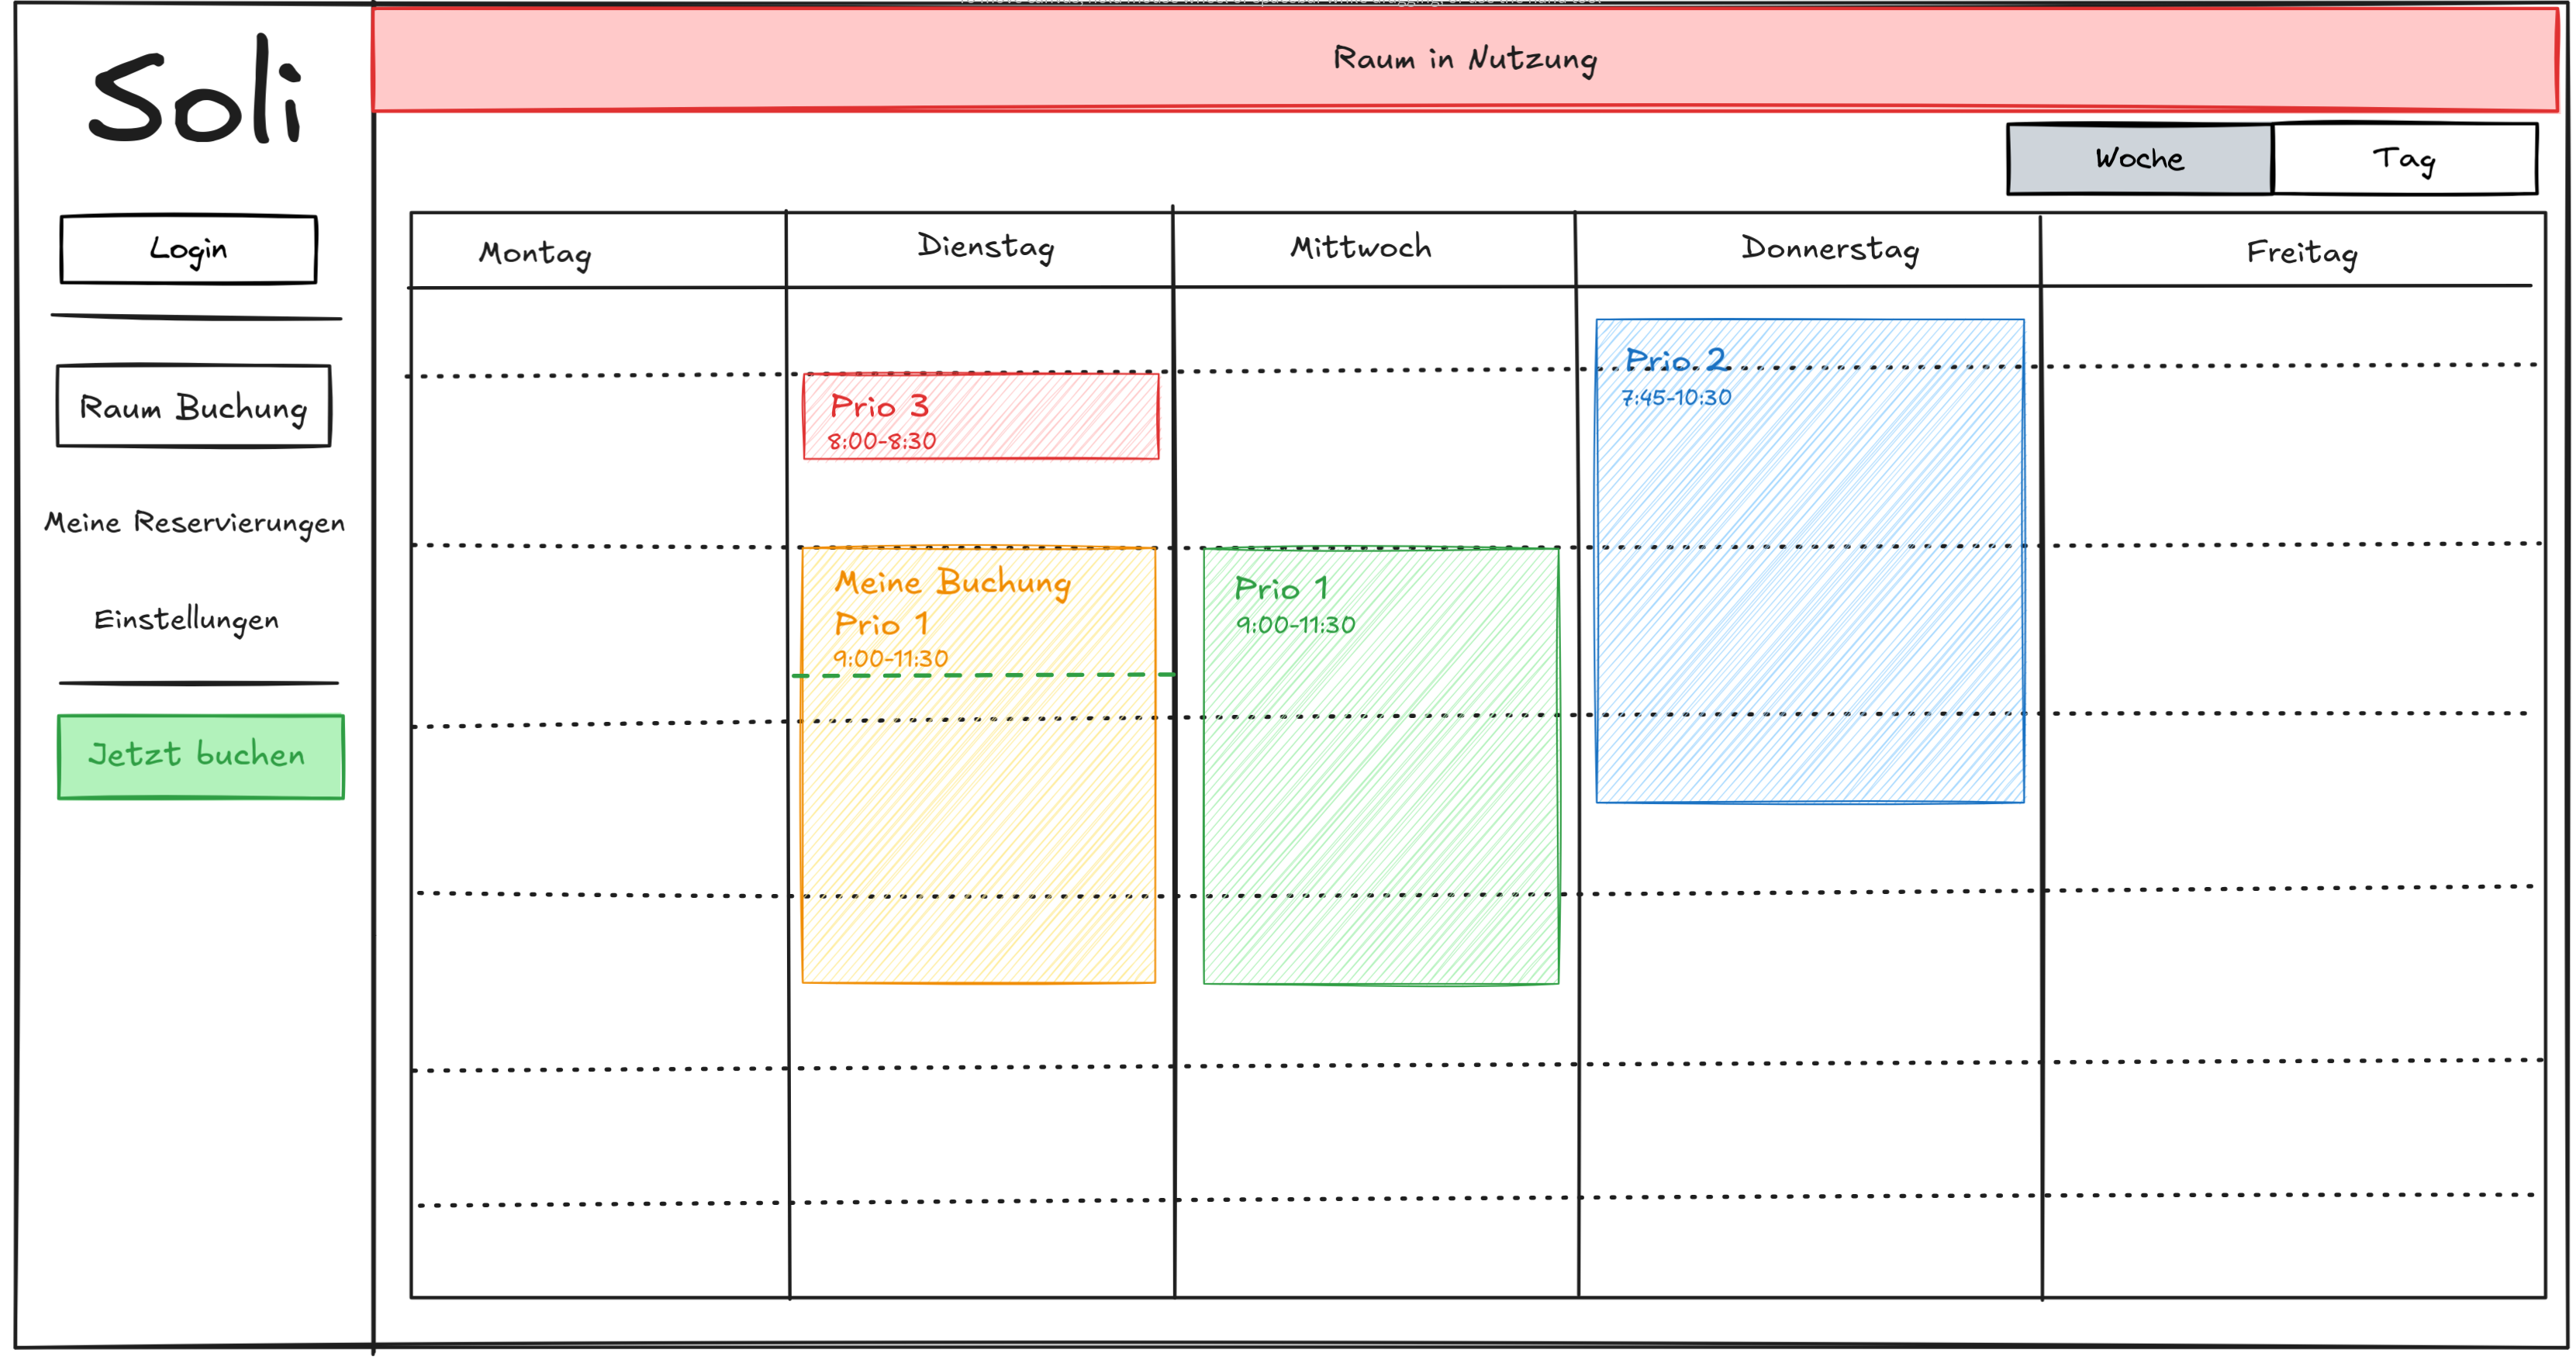
\includegraphics[scale=0.15]{figures/ui/startseite}
    \caption{Startseite der Anwendung}
    \label{fig:startseite}
\end{figure}
\clearpage

Sollten NuterInnen eine Buchung vornehmen wollen, so klicken diese in den gewünschten Zeitraum
und es wird der Dialog in \ref{fig:buchung} dargestellt.
Hier können NutzerInnen die gewünschte Zeit und den Raum auswählen.
\begin{figure}[ht]
    \centering
    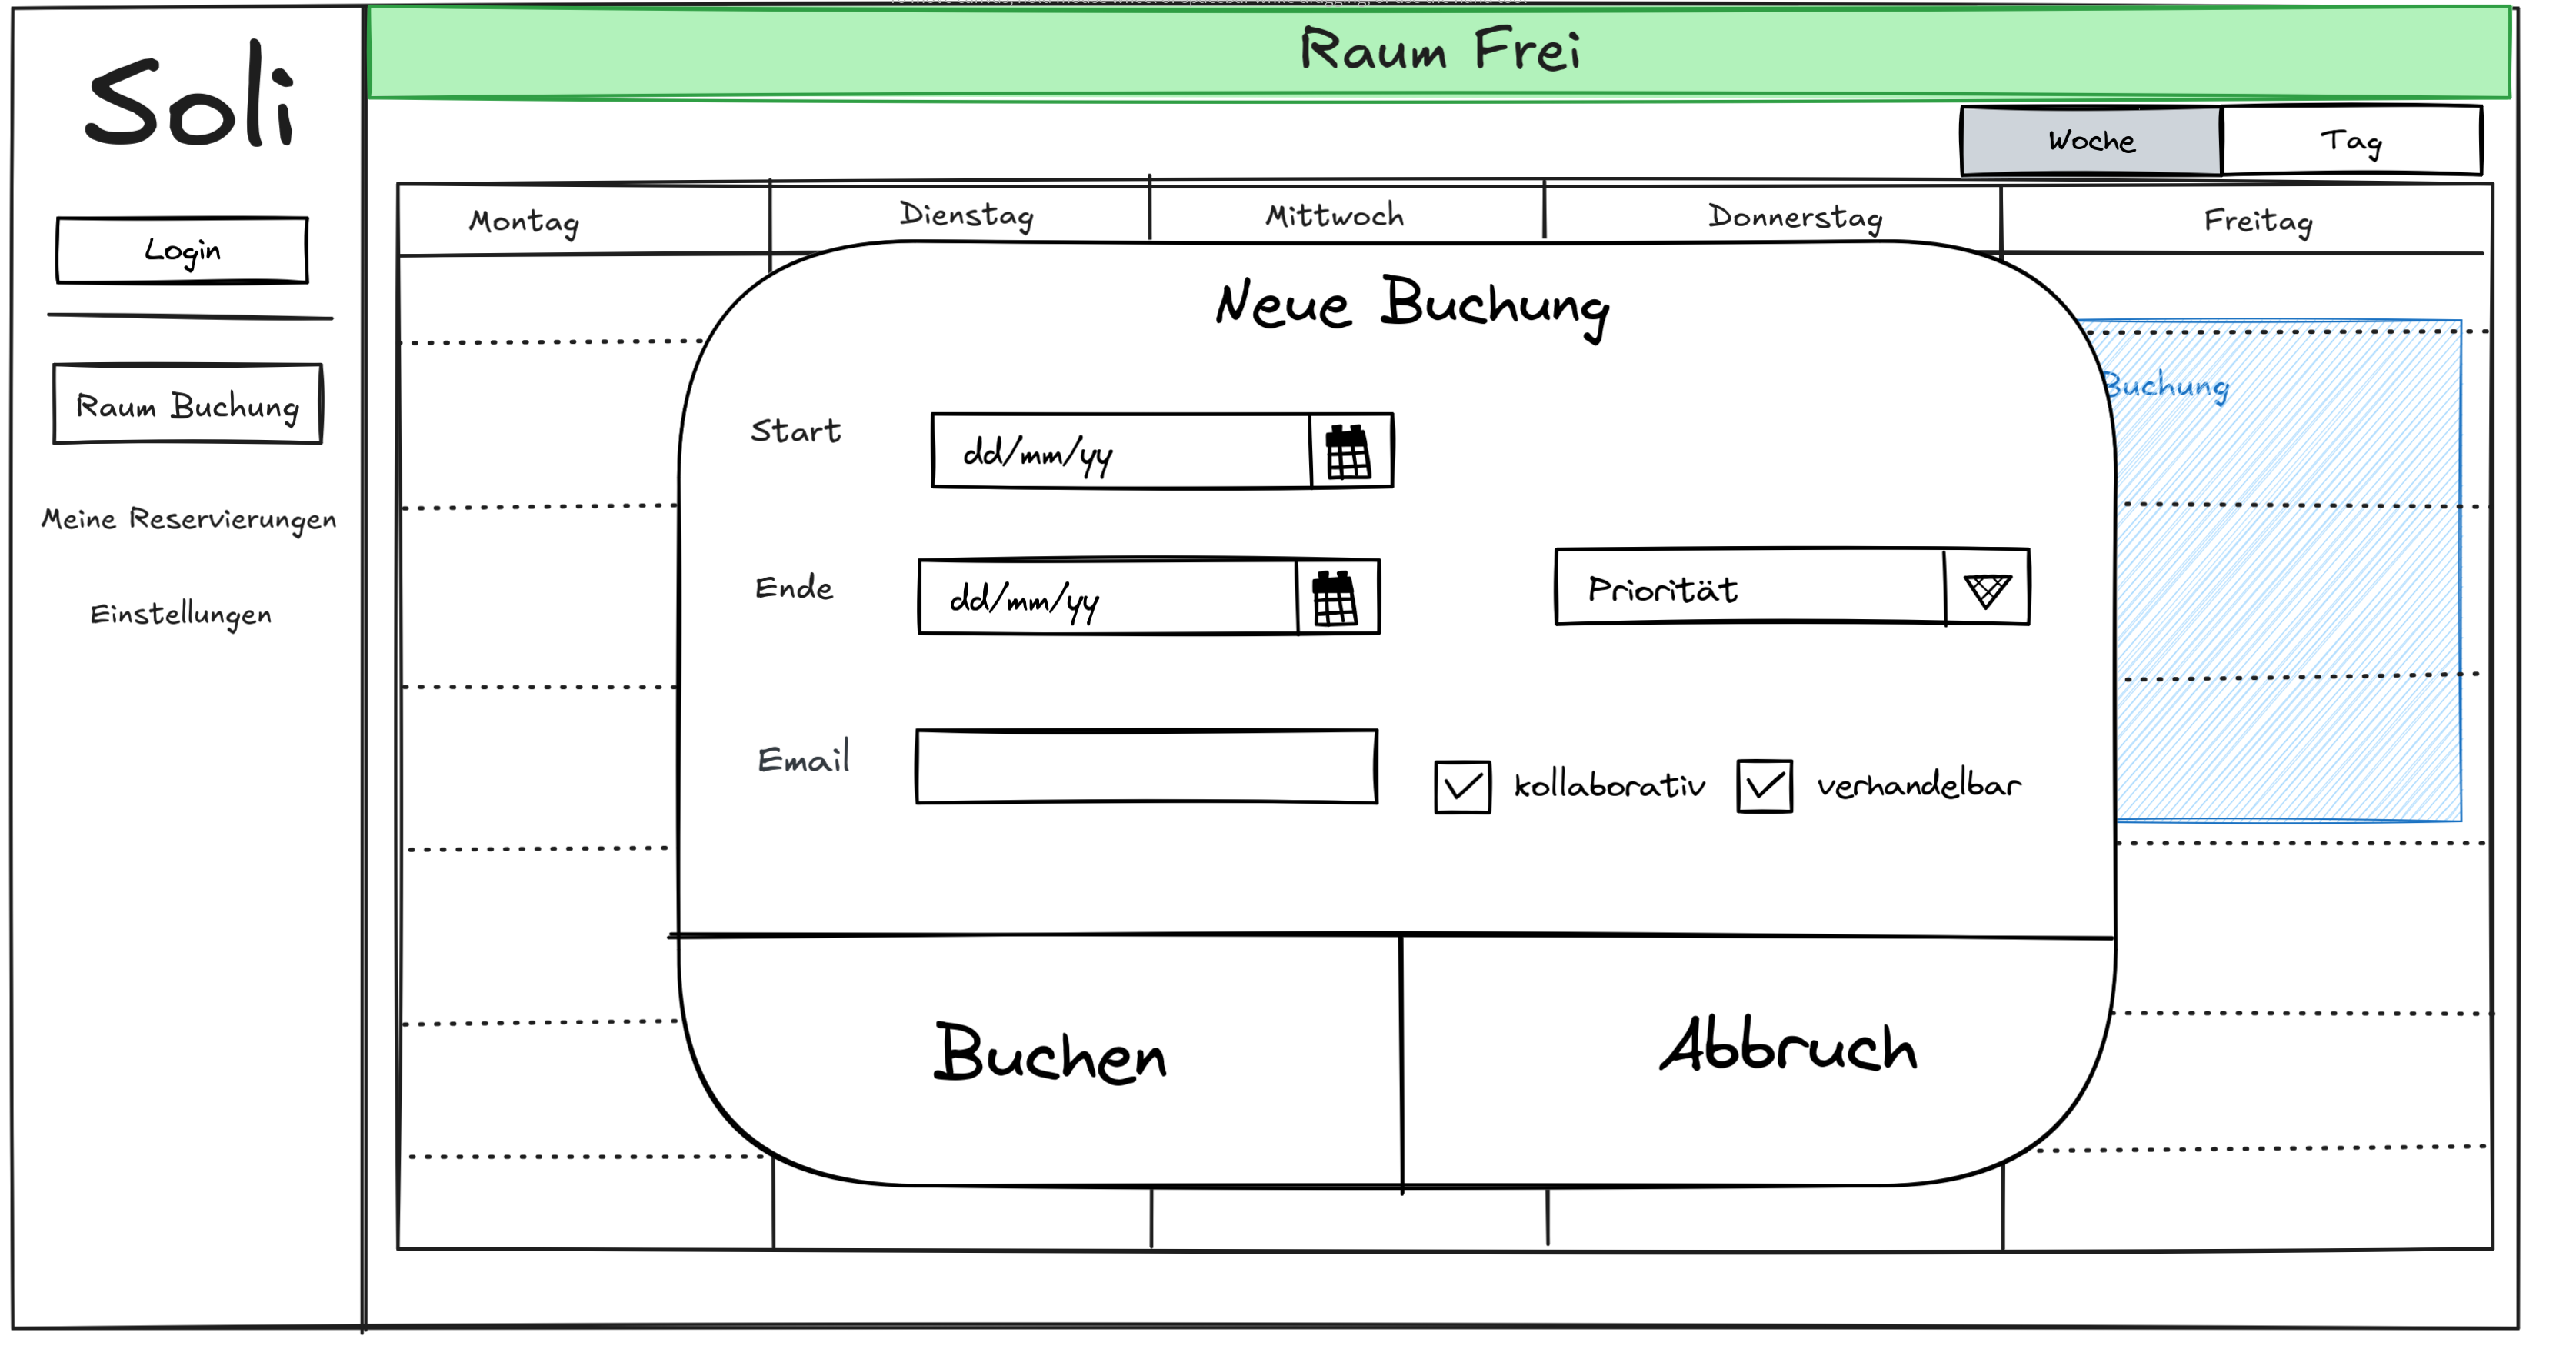
\includegraphics[scale=0.15]{figures/ui/buchungsdialog}
    \caption{Buchungsdialog}
    \label{fig:buchung}
\end{figure}
\clearpage

Tätigen NutzerInnen eine Buchung, so werden diese aufgefordert, sich anzumelden.
Der hierzu gehörige Dialog ist in \ref{fig:login} dargestellt.
Alternativ ist dieser Dialog auch über den Anmeldungsbutton, der in Abbildung \ref{fig:startseite} zu sehen ist, erreichbar.
\begin{figure}[ht]
    \centering
    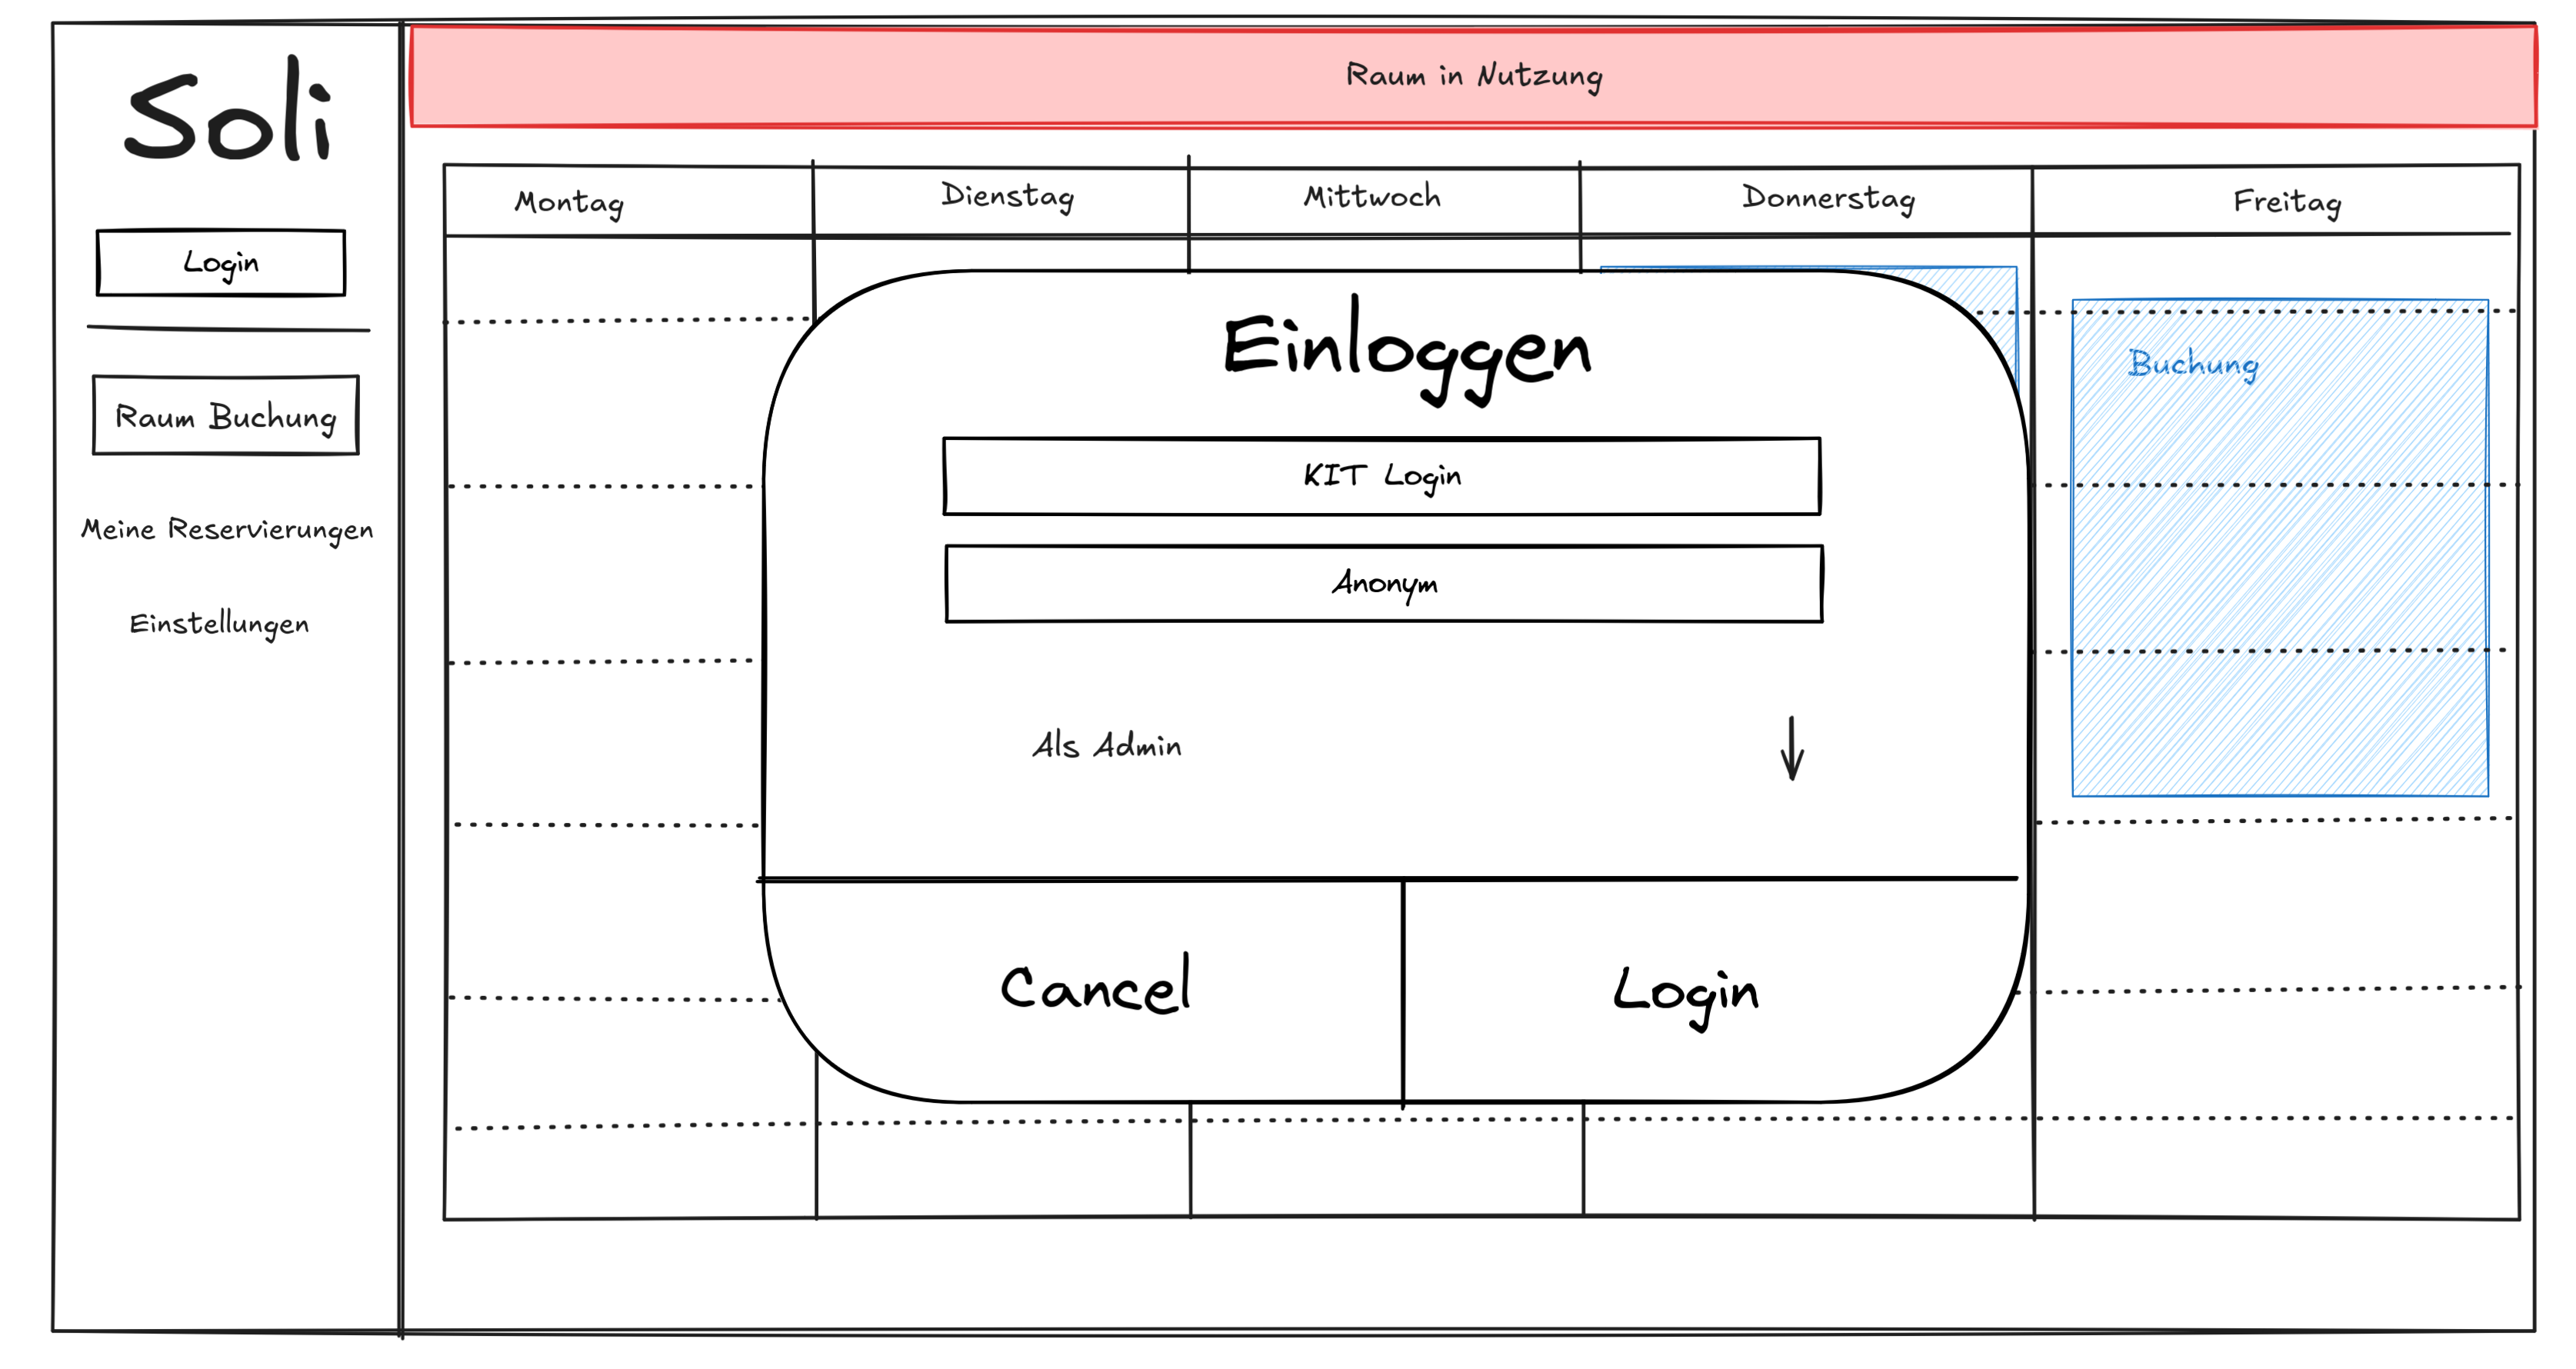
\includegraphics[scale=0.15]{figures/ui/anmeldungsseite}
    \caption{Anmeldungsseite}
    \label{fig:login}
\end{figure}
\clearpage

Sind NutzerInnen eingeloggt und belegen den Raum,
so wird ihnen die in Abbildung \ref{fig:checkout} dargestellte Ansicht angezeigt.
Hier können NutzerInnen den Raum wieder über den Quick-Checkout Button freigeben.
\begin{figure}[ht]
    \centering
    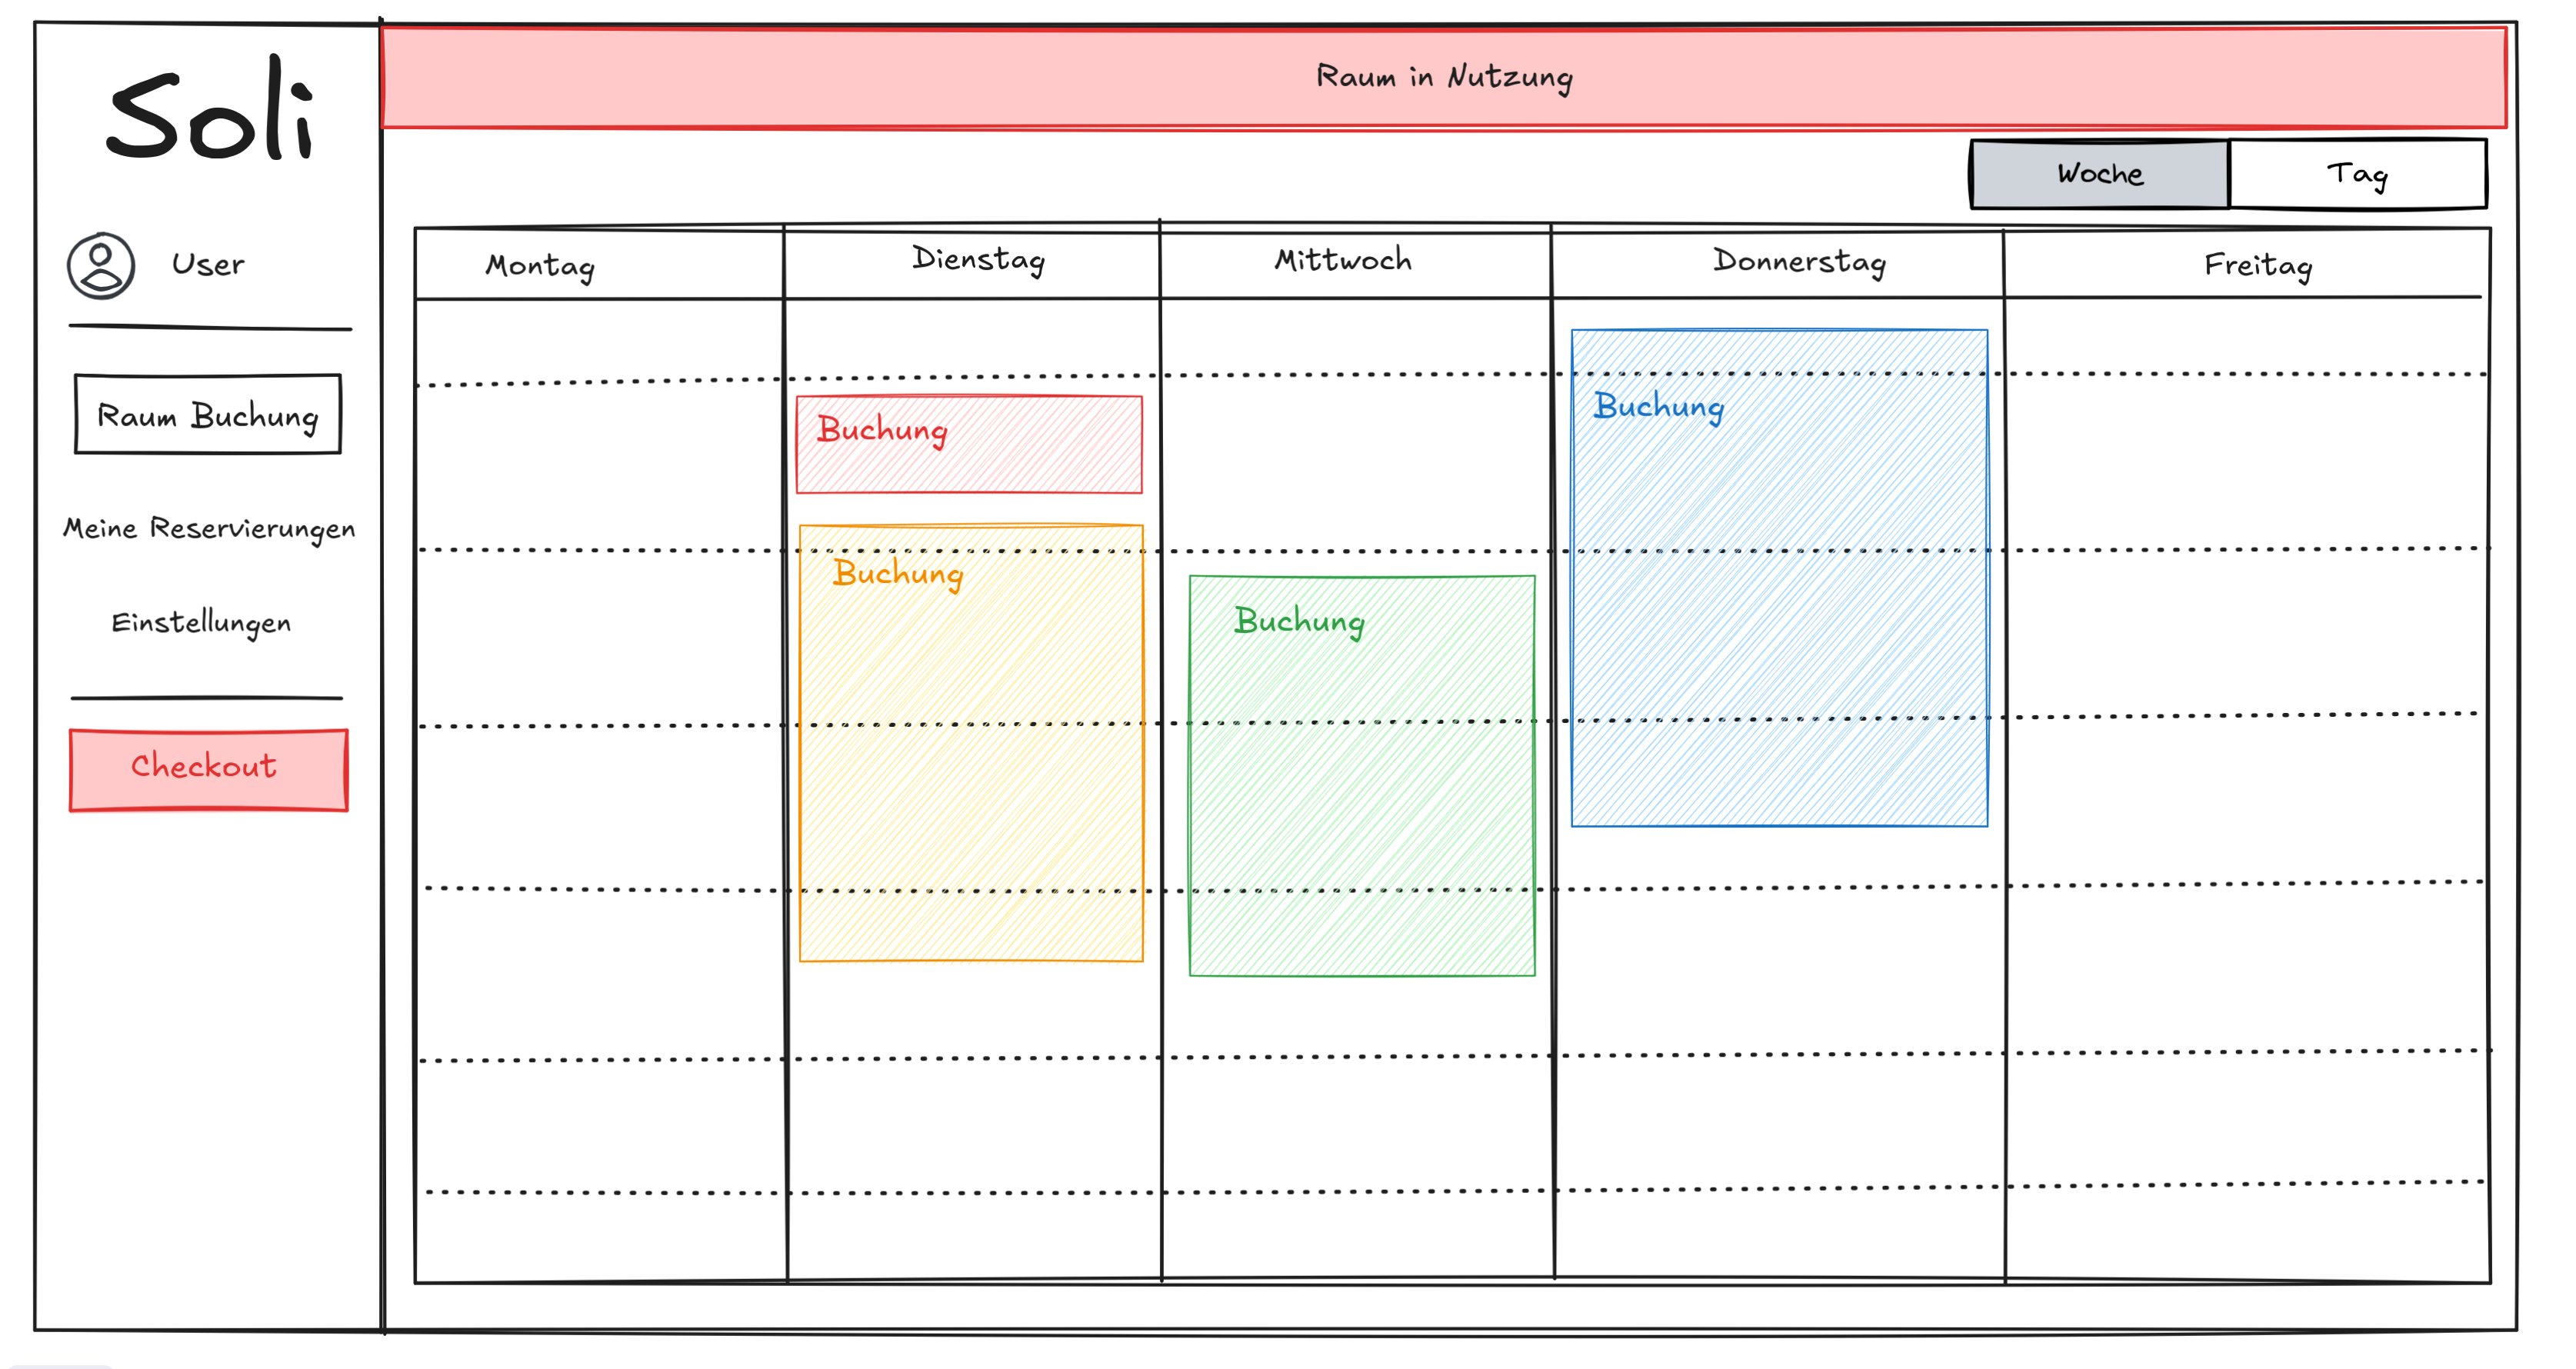
\includegraphics[scale=0.15]{figures/ui/checkout}
    \caption{Quick Checkout}
    \label{fig:checkout}
\end{figure}
\clearpage

\section{Buchungsverwaltung}
Sollte ein Benutzer eine Buchung vorgenommen haben, so kann dieser in der Reservierungsübersicht,
die in Abbildung \ref{fig:overview} dargestellt ist, seine Buchungen einsehen und verwalten.

\begin{figure}[ht]
    \includegraphics[scale=0.15]{figures/ui/reservierungsübersicht}
    \caption{Reservierungsübersicht}
    \label{fig:overview}
\end{figure}
\clearpage

\section{Adminstration}
Ein Adminitrator hat die Möglichkeit, über die Benutzeradminstrationsoberfläche,
die in Abbildung \ref{fig:adminuser} dargestellt ist, NutzerInnen einzusehen und zu verwalten.
So dient diese Ansicht z.B. dazu, NuterInnen zu sperren oder zu entsperren.

\begin{figure}[ht]
    \centering
    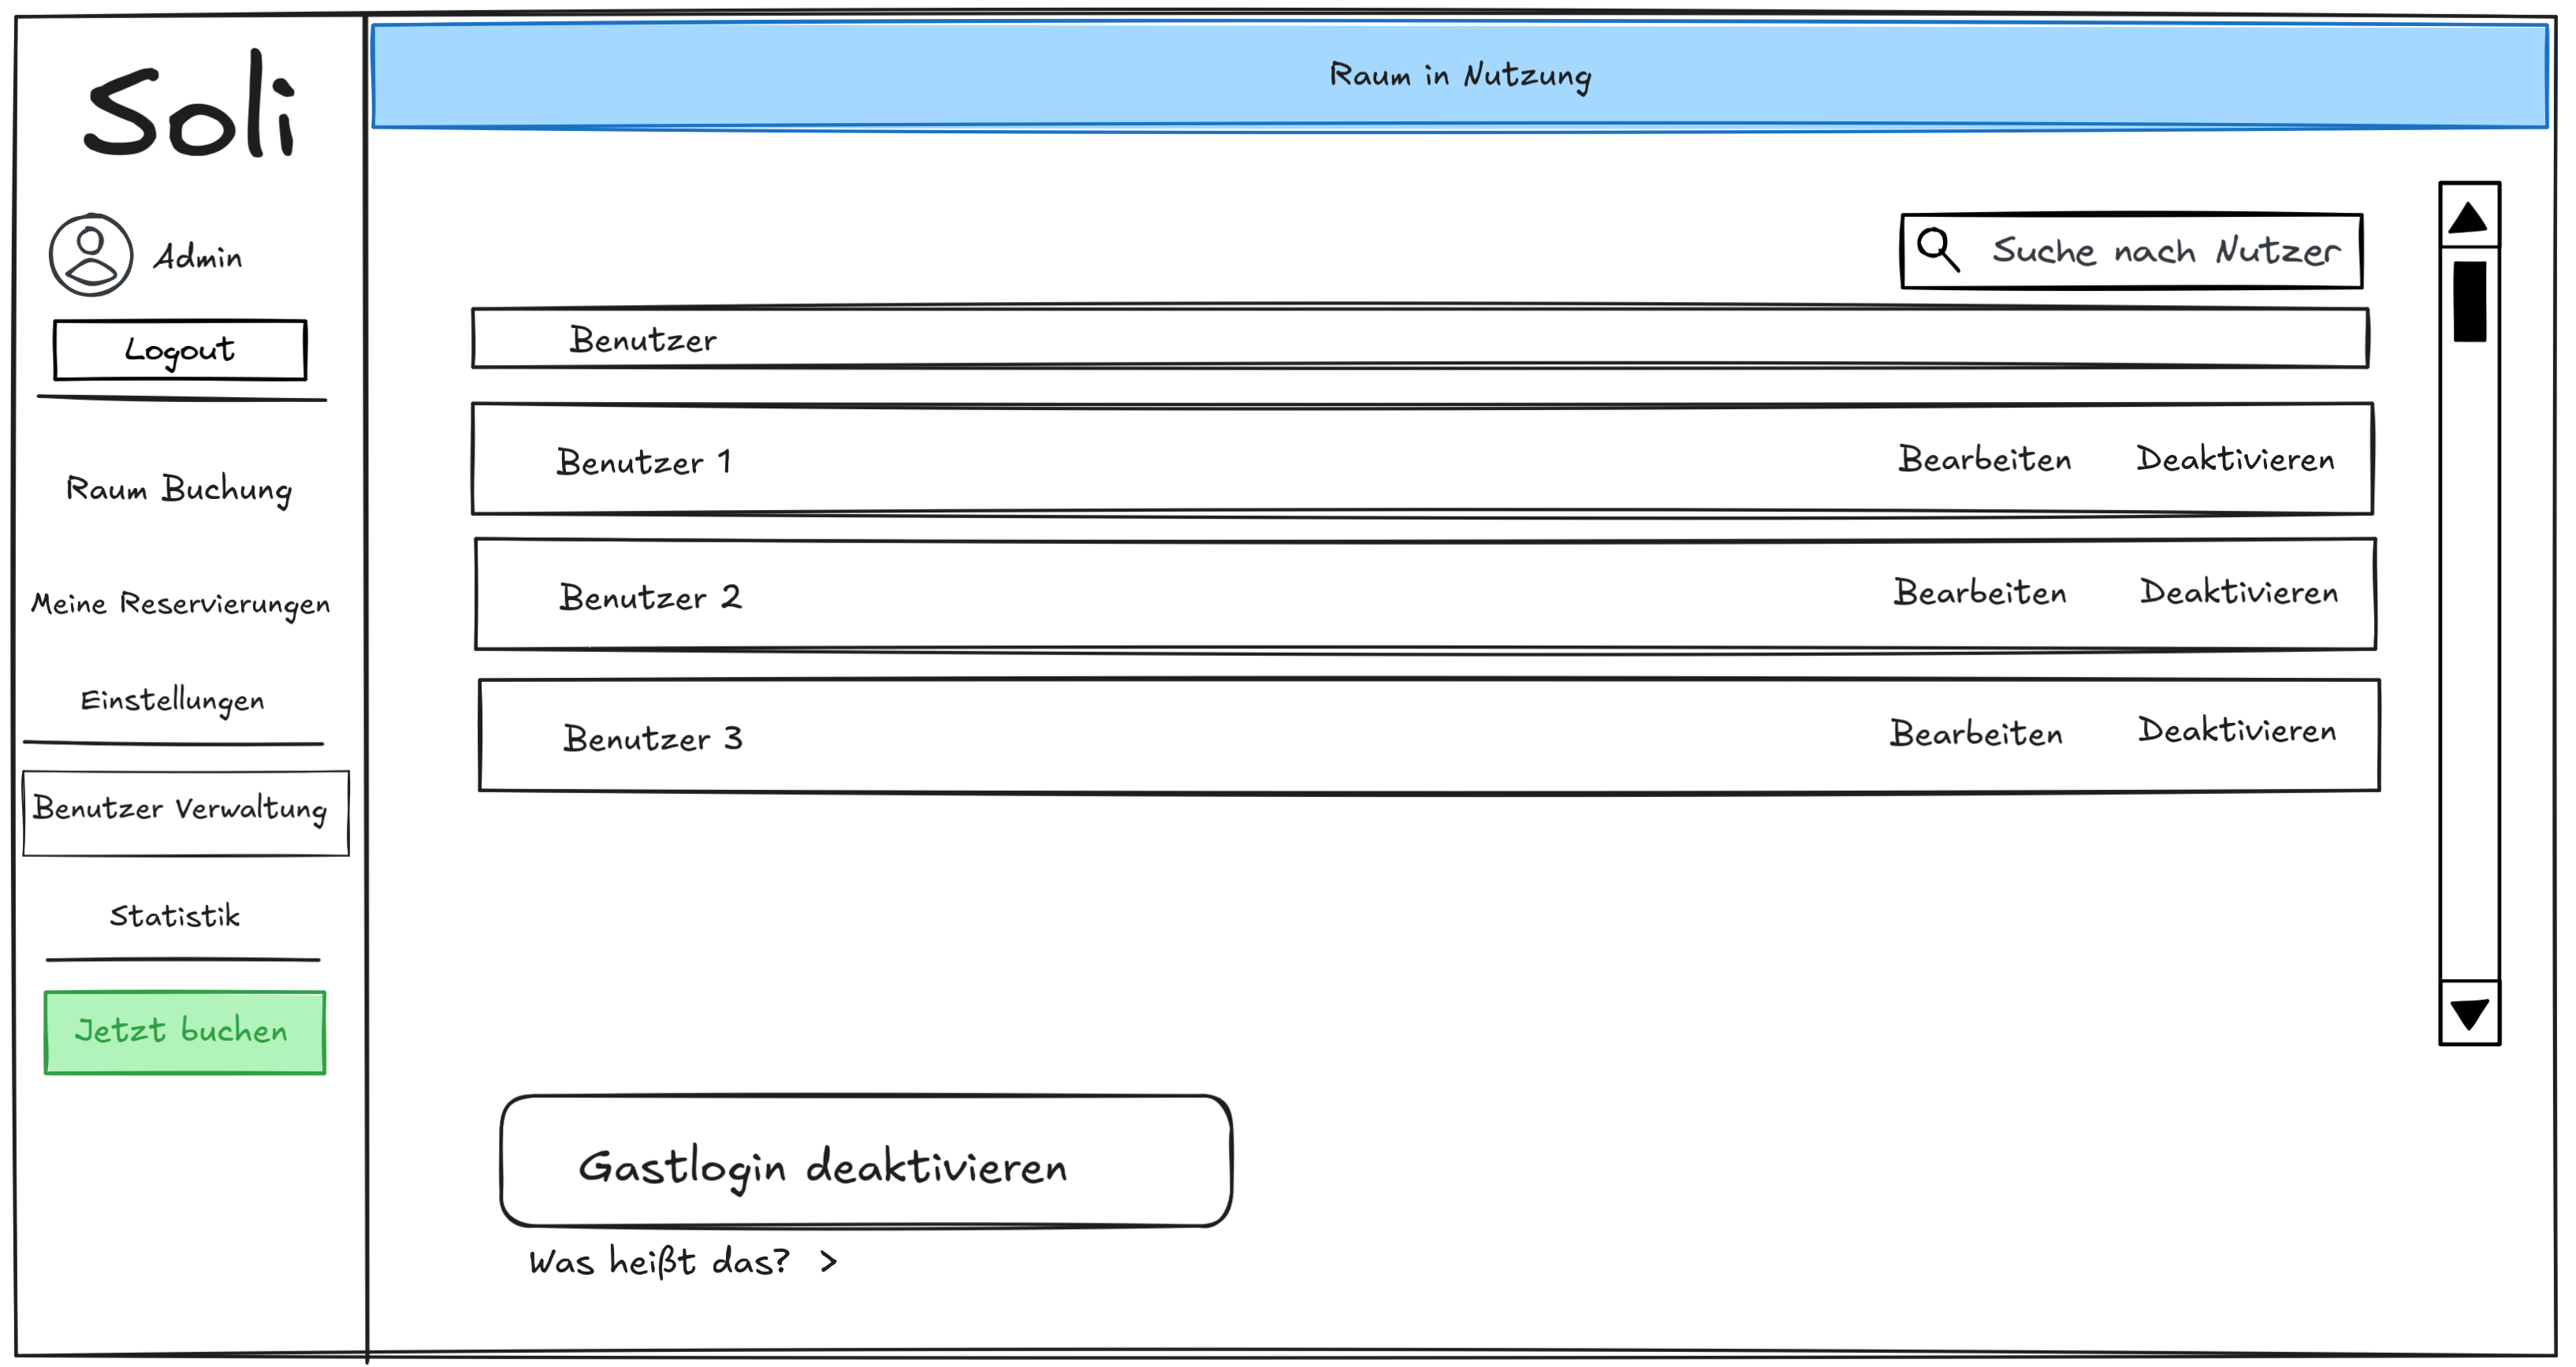
\includegraphics[scale=0.15]{figures/ui/useradminui}
    \caption{Benutzeradminstrationsoberfläche}
    \label{fig:adminuser}
\end{figure}

